documentclass{article}
\usepackage[utf8]{inputenc}
\usepackage{graphicx}
\usepackage{hyperref}
\title{Herramientas para la minería de datos}
\author{Rodrigo Reyes M.}
\date{}
\begin{document}

\maketitle

\section{¿Qué es ETL?}
El término ETL es comúnmente la abreviatura de \textit{Extraction, Transformation , Loading}, veamos a detalle los tres procesos.
\begin{itemize}
\item Extraction : En múltiples ocasiones se requiere obtener de diversas fuentes datos en distintos formatos y dimensionalidad.Ësto supone un problema de extraer y juntar de éstas fuentes para intgrarlos a una base de datos.
\item Transformation : Como se ha visto en diversos escenrios es necesario traducir ó transformar la información antes de guardarla en una base de datos.
\item Loading es la fase en la cual se cargan a la base de datos o el almacén de datos (que se verá más adelante) aqui se pueden ejecutar programas de monitoreo o de historial de consultas.
\end{itemize}

Existen diversas herramientas que permiten realizar ETL, como por ejemplo:
\begin{itemize}
\item Kettle
\item OWB (Oracle Warehouse Builder) y ODI (Oracle Data Integrator)
\item Talend
\item SSIS (Microsoft)
\end{itemize}
\section{¿Qué es un DataWarehouse (Almacén de Datos)?}
Tradicionalmente las bases de datos utilizan un esquema normalizado, esto permite evitar redundancia en los datos.
Sin embargo, existe una clara desventaja que al tener la información en distintas tablas las consultas resultan bastante complejas y costosas
en términos de memoria y de tiempo de procesamiento.
De ahí surge el concepto de replantear la arquitectura de las bases de datos.
La arquitectura más común en DW es el diseño en forma de estrella.
Aquí un ejemplo de dicho modelo.
\begin{figure}[h]
\centering
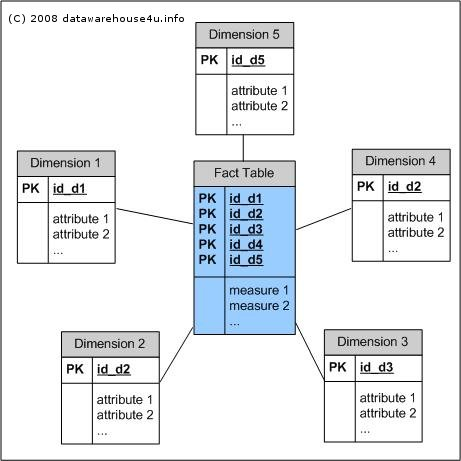
\includegraphics[width=7cm, height=7cm]{star_schema.jpg}
\caption{Modelo estrella de un almacén de datos.}
\label{fig:my_label}
\end{figure}
Como se puede observar hay una tabla central llamada \textit{Fact Table} y varias tablas alrededor llamadas \textit{dimensiones}.
La tabla central generalmente contiene medidas o métricas de un evento en específico.Es decir los registros en ésta tabla central están normalizados en su tercer forma normal (3NF), además contiene Llaves foráneas que se conectan a las tablas dimensionales.
Las tablas adyacentes se les conoce como dimensiones, contienen atributos acerca de las llaves primarias de la tabla de \textit{facts}, las llaves primarias de éstas son las llaves foráneas compuestas de la tabla de \textit{facts}.
\subsection{Ejercicios}
\begin{enumerate}
\item Realiza un esquema de almacén de datos con el diseño en forma de estrella.(Puede ser inventando o con un esquema real de base de datos)
\item Investiga, ¿Cómo es el diseño en forma de copo de nieve \textit{Snowflake}?
\item ¿Cuáles son las ventajas y desventajas de los dos esquemas \textit{Snowflake} y \textit{Star}?
\end{enumerate}
\section{MapReduce}

Ahora veremos uno de los procesos más comunes al tratar grandes cantidades de datos.Se le conoce como \textit{MapReduce} son dos palabras que se prodrían traducir a mapeo-reducción, se distinguen tres procesos:
\begin{enumerate}
\item Mapeo : Obtiene de un archivo o de un \textit{pipeline} y mapea a las llaves y valores que se utilizaran en el siguiente paso.
\item Ordenamiento o \textit{Shuffle} : Aqui se utilizan las llaves-valor del paso anterior para ordenar o realizar operaciones que optimicen el siguiente paso.
\item Reducción: En éste proceso se utilizan agrupamientos o funciones de los valores mapeados, generalmente reducen la cardinalidad de las entradas.
\end{enumerate}
Muchos de éstos algoritmos se ejecutan en paralelo, el software más común para ésto es \textit{Hadoop}.

\section{Cubos OLAP (OnLine Analytical Processing)}
Los almacenes de datos nos permiten construir varias herremientas que analizan e utilizan los datos.Un ejemplo muy útil son los cubos OLAP, los cubos surgen debido a la necesidad de consultar,visualizar y analizar los datos de un almacén.Entonces, los cubos OLAP son una especie de interfaz mediante la cual se pueden realizar consultas llamadas \verb#MDX queries# que signifca \verb#MultiDimensional eXpressions#.En ocasiones la literatura llama a éstos hipercubos por considerarse cubos de dimensiones superiores a 3.
Existen 2 variaciones de los cubos OLAP:
\begin{enumerate}
\item MOLAP : Multidimensional OLAP, se guarda en arreglos densos.(o bases NoSQL)
\item ROLAP : Relational OLAP. se guarda en bases de datos relacionales.
\end{enumerate}
\begin{figure}[h]
\centering
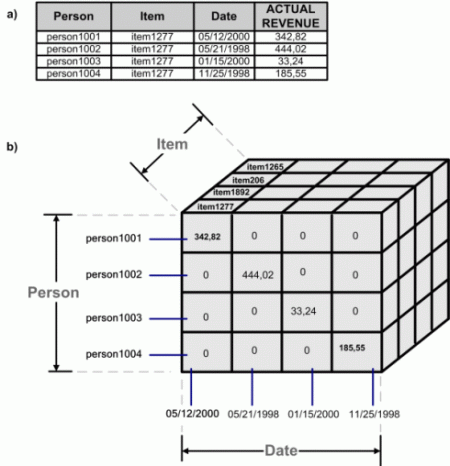
\includegraphics[width=7cm, height=7cm]{OLAP-vs-Table.png}
\caption{a) Una tabla tradicional b) Visto desde la abstracción de un cubo OLAP}
\label{fig:my_label}
\end{figure}

\section{Ejercicios}
\begin{enumerate}
\item Investiga en el sitio de Mondrian  \url{http://mondrian.pentaho.com/documentation/} y escribe en un reporte de aproximadamente 2 cuartillas acerca de la herramienta.
\item Indica un uso que le darías a ésta herramienta.
\end{enumerate}

\end{document}
